%++++++++++++++++++++++++++++++++++++++++
% Don't modify this section unless you know what you're doing!
\documentclass[letterpaper,12pt]{article}
\usepackage{tabularx} % extra features for tabular environment
\usepackage{amsmath}  % improve math presentation
\usepackage{graphicx} % takes care of graphic including machinery
\usepackage{subfig}
\usepackage{subfloat}
\usepackage[margin=1in,letterpaper]{geometry} % decreases margins
\usepackage{cite} % takes care of citations
\usepackage[final]{hyperref} % adds hyper links inside the generated pdf file
\hypersetup{
	colorlinks=true,       % false: boxed links; true: colored links
	linkcolor=blue,        % color of internal links
	citecolor=blue,        % color of links to bibliography
	filecolor=magenta,     % color of file links
	urlcolor=blue         
}
%++++++++++++++++++++++++++++++++++++++++


\begin{document}

\title{Detection and localization of a 2-D contour with GHT}
\author{E. Hyrol and P. Stiasny}
\date{22.01.2017}
\maketitle

%\begin{abstract}
%
%\end{abstract}


\section{Introduction}

In the scope of this project a complete application capable of template detection via Generalized Hough Transform will be implemented. The goal is to understand the algorithm, experiment with different parameters and observe how it performs.

\section{Theory}

\subsection{Image edge detection}

A pre-processing step in edge detection: a smoothing operation in order to remove noise (spiky-like variations) from the image.


\begin{figure}[!th]
  \centering
  \subfloat[Desired edge.]{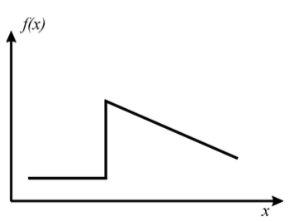
\includegraphics[width=0.4\textwidth]{desired_edge}\label{fig:d_edge}}
  \hfill
  \subfloat[Real edge.]{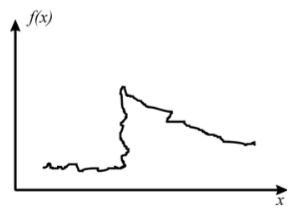
\includegraphics[width=0.4\textwidth]{real_edge}\label{fig:r_edge}}
  \caption{Example edges.}
\end{figure}

\textbf{Basic types of image edge detectors: }

\begin{itemize}
	\item discrete image function gradients
	\item convolution kernels
 	\item using parametric edge models
 	\item mixed approaches

\end{itemize}


\subsection{Sobel Edge Detection}

The Sobel operator is used in image processing, particularly within edge detection algorithms. It falls into a group of convolution-based edge detectors. Technically, it is a discrete differentiation operator, computing an approximation of the gradient of the image intensity function. At each point in the image, the result of the Sobel operator is either the corresponding gradient vector or the norm of this vector. The Sobel operator is based on convolving the image with a small, separable, and integer valued filter in horizontal and vertical direction and is therefore relatively inexpensive in terms of computations. On the other hand, the gradient approximation that it produces is relatively crude, in particular for high frequency variations in the image.

\[	
  	\Delta x = \begin{bmatrix}
  	-1 & 0 & 1 \\
  	-2 & 0 & 2 \\
  	-1 & 0 & 1
	\end{bmatrix}, \quad
	\Delta y = \begin{bmatrix}
  	1 & 2 & 1 \\
  	0 & 0 & 0 \\
  	-1 & -2 & -1
	\end{bmatrix}
\]

\textbf{Characteristics:} different input-output image, e.g. maximum strength: 2040 for 8-bit input image, simple implementation, good results.


\subsection{Edge thinning}

\textbf{Threshold-based edge elimination.} This simple edge thinning method is an edge elimination operator with a minimum threshold parameter $\theta$. The threshold is either fixed or set adaptively (e.g. $\theta = \gamma S_{max}$, where $ \gamma \in(0,1)$).

\begin{equation}
s_{thin}(P) = \begin{cases}
	s(P), & \text{if}\ s(P) > \theta	\\
	0, & \text{otherwise}
\end{cases}
\label{ncc}
\end{equation}

\textbf{No-maximum edge elimination.} It depends on a check in the local neighborhood of given pixel P:

\begin{gather}
	IF(s(P)\geq s(N_L) OR |r(P)-r(N_L)|\geq T)\
	AND\ (s(P)\geq s(N_R)OR |r(P)-r(N_R)|\geq T)\\
	THEN s(P)_{THIN}=s(P):
	ELSE s(p)_{THIN}=0;
\end{gather}

\begin{figure}[!th]
  \centering
  {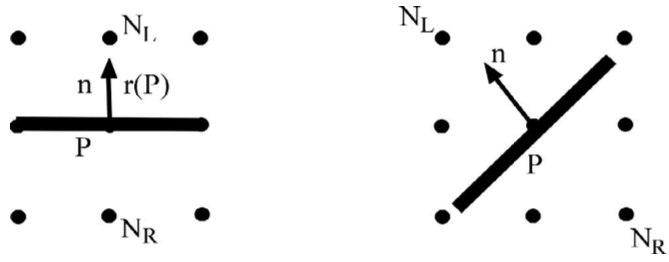
\includegraphics[width=0.6\textwidth]{edge_thin_neghb}\label{fig:edge_thin_n}}
    \caption{No-maximum edge elimination.}
  \end{figure}


\textbf{Edge modification.}A local neighborhood-based modification of edge at pixel P:
\begin{itemize}
	\item if P is the strongest edge element in the set: P, NL, NR , then:
\[ s^{'} (P)=s(P)+ \alpha(s(N_L)+s(N_R ))\]
	\item if P is the weakest edge element in the above set then:
\[s^{'}(P) = s(P) - 2 \alpha s(P) \]
	\item if one neighbour of P (denoted by $P^+$ ) is a stronger edge and another neighbour of P (denoted by $P^-$ ) is a weaker edge element then:
\[s^{'}(P) = s(P) - \alpha s(P^+) + \alpha s(P^-).\]
\end{itemize}

Several iterations over the whole image may be necessary.\\

\textbf{Edge elimination with hysteresis threshold.} This edge thinning method works with two edge strength thresholds: \textbf{the upper $\theta_H$} and \textbf{the lower $\theta_L$}.
In the first run these edge pixels are individually marked as "good" that have higher strengths than the upper threshold.
In the next run these "good" pixels are tried to be “extended” along a potential contour line in both directions (“positive” and “negative” line direction). For a single extension, the neighbour pixel needs to have a higher strength than the lower threshold.

\underline{Remark:} Now the neighbours are not competing with each other and they are searched along the expected contour line (not across it).


\subsection{Edge chain following}

\underline{Principle:} searching for extension of current edge pixel $P=P_{-cur}$ by its successor edge $N=c(P_{cur})$.
Two neighbour edge elements can be linked if the edge magnitude (strength) and direction differences are below certain thresholds and their magnitudes are relatively large:

\begin{gather}
	|s(P)-s(N)|\leq T_1 \\
	|r(P)-r(N)|\ mod\ 2\pi\leq T_2 \\
	|s(P)|>T,\ |s(N)|>T
\end{gather}

Denote the 3 nearest pixel along the direction $r(P)$ as: $N_1, N_2, N_3$. The successor of $P_{-cur}$: an edge element Ni whose strength and
 orientation are most similar to $P_{-cur}$.

\textbf{Successor candidates}. Three candidates for a successor of pixel P:

\begin{figure}[!th]
  \centering
  {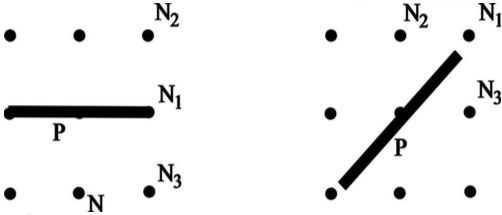
\includegraphics[width=0.5\textwidth]{succ_cand1}\label{fig:succ_cand1}}
%    \caption{No-maximum edge elimination.}
  \end{figure}

Closing a gap for edge pixel P in directions (left) $0^\circ$ and (right) $45^\circ$:
\begin{figure}[!th]
  \centering
  {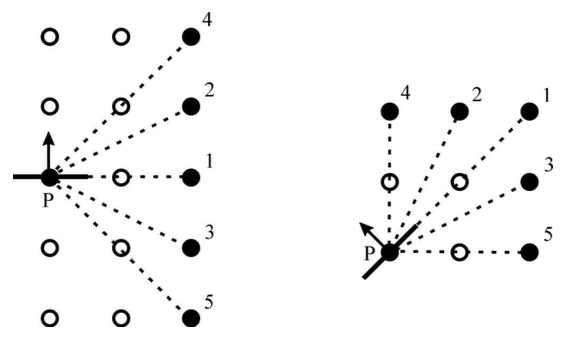
\includegraphics[width=0.5\textwidth]{succ_cand2}\label{fig:succ_cand2}}
%    \caption{No-maximum edge elimination.}
  \end{figure}
  
  
\textbf{The hysteresis threshold method}.
Contrast (edge strength) may be different in different points of the contour. Careful thresholding of $M(x,y)$ is needed to remove  weak edges while preserving the connectivity of the contours.

Hysteresis thresholding receives the output of the non-maxima suppression, $M_{NMS}(x,y)$.

The algorithm uses 2 thresholds, $T_{high}$ and $T_{low}$:

\begin{itemize}
	\item A pixel $(x,y)$ is called strong if $M_{NMS}(x,y) > T_{high}$.
	\item A pixel $(x,y)$ is called weak if $M_{NMS}(x,y) \leq T_{low}$.
	\item All other pixels are called candidate pixels.
\end{itemize}

The algorithm has the following steps:
\begin{enumerate}


	\item  In each position of $(x,y)$, discard the pixel $(x,y)$ if it is weak; output the pixel if it is strong.
	\item If the pixel is a candidate, follow the chain of connected local maxima in both directions along the edge, as long as $M_{NMS}(x,y) > T_{low}$.
	\item If the starting candidate pixel $(x,y)$ is connected to a strong pixel, output this candidate pixel; otherwise, do not output the candidate pixel.
\end{enumerate}

An example can be observed on Figure \ref{fig:edge_chain_labs}.

\begin{figure}[!th]
  \centering
  {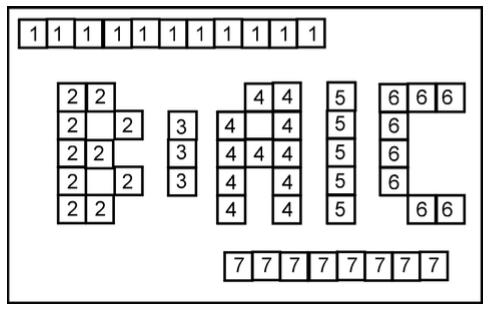
\includegraphics[width=0.5\textwidth]{edge_chain_labs}}

    \caption{Edge chain labels  	\label{fig:edge_chain_labs}}
  \end{figure}


\subsection{Generalized Hough Transform}


To generalize the Hough algorithm to non-analytic curves,  Dana H. Ballard defines the following parameters for a generalized shape: $a={y,s,θ}$, where $y$ is a reference origin for the shape, $\theta$ is its orientation, and $s = (sx, sy)$ describes two orthogonal scale factors. As in the case of initial Hough Transforms, there is an algorithm for computing the best set of parameters for a given shape from edge pixel data. These parameters no longer have equal status. The reference origin location $y$ is described in terms of a template table called the \textbf{R-table} of possible edge pixel orientations. The computation of the additional parameters s and $\theta$ is then accomplished by straightforward transformations to this table. The key to generalizing the Hough algorithm to arbitrary shapes is the use of directional information. Given any shape and a fixed reference point on it, instead of a parametric curve, the information provided by the boundary pixels is stored in the form of the R-table in the transform stage. For every edge point on the test image, the properties of the point are looked up on the R-table and reference point is retrieved and the appropriate cell in a matrix called the \textbf{Accumulator matrix} is incremented. The cell with maximum 'votes' in the \textbf{Accumulator matrix} can be a possible point of existence of fixed reference of the object in the test image.

%\textbf{Parameters of the Hough space:} $C = (x_C; y_C)$: location of the center mass, $s$ - scale, $\alpha$ - contour orientation angle.
%
%\textbf{Model learning (design).} For every pair of allowed discrete values $s_d$, $\alpha_g$ of scale and orientation, create a table $R(s_d, \alpha_g) = [ r( \varphi ), \varphi ]$, where for each
%edge $x_B$ with edge direction $\varphi$ the pair:
%$[r(\varphi)=x_B - C, \varphi]$ is stored.


\begin{figure}[h]
  \centering
  \subfloat[Model contour.]{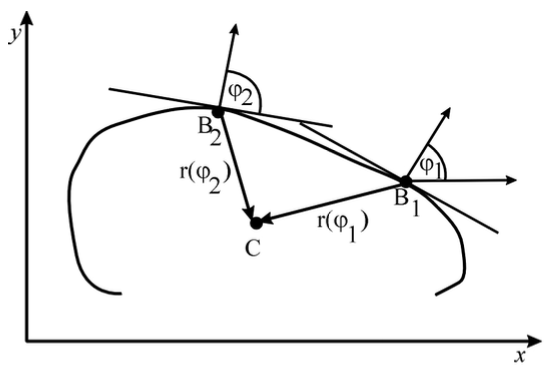
\includegraphics[width=0.4\textwidth]{ght_model_cont}\label{fig:ght_model_cont}}
  \hfill
  \subfloat[Candidate contour.]{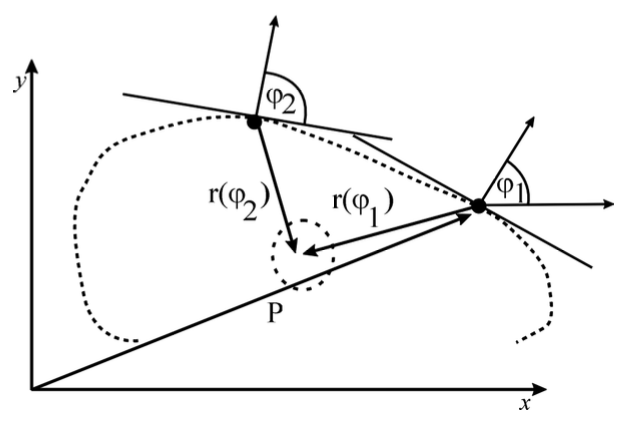
\includegraphics[width=0.4\textwidth]{ght_candid_cont}\label{fig:ght_candid_cont}}
  \caption{Example of GHT contour detection.}
\end{figure}

\subsection{Building the R-Table}

First a reference point $y$ inside the shape should be chosen. Next for each boundary point $x$ $\phi(x)$, gradient direction and $r = y – x$ should be computed. $r$ should be stored as a function of $\phi$. Notice that each index of $\phi$ may have many values of $r$. One can either store the co-ordinate differences between the fixed reference and the edge point $((x_c – x_{ij}),( y_c - y_{ij}))$ or as the radial distance and the angle between them $(r_{ij} , \alpha_{ij})$. Having done this for each point, the R-table will fully represent the template object. Also, since the generation phase is invertible, it may be used to localise object occurrences at other places in the image.


\subsection{Object localization}

For each edge pixel x in the image, the gradient $\phi$  should be found and all the corresponding points $x+r$ in the accumulator array A (initialized to a maximum size of the image)should be incremented, where $r$ is a table entry indexed by $\phi$, i.e., $r(\phi)$. These entry points provide each possible position for the reference point. 

Simple transformations of the R-table will allow to detect scaled and rotated instances of the template. For example if the shape is scaled by $s$ and this transformation is denoted by $T_s$, then

\[T_s[R(\phi)]=sR(\phi) \]

i.e. all the vectors inside R-table are scaled by $s$. Also if the object is rotated by $\theta$ and this transformation is denoted by $T_\theta$, then

\[T_\theta[R(\phi)]=Rot\{R(\phi-\theta)mod2\pi],0\} \]

i.e. all the indices are incremented by - $\theta 
 modulo 2\pi$, the appropriate vectors are found and then they are rotated by $\theta$. 
Although some bogus points may be calculated, given that the object exists in the image, a maximum will occur at the reference point. Maxima in A correspond to possible instances of the shape.

\section{Project implementation}


For implementation we chose the Python programming language and used the NumPy library
for efficient matrix operations.  We also used scikit and scikit-image for required
matrix operations not found in NumPy.  Slow hotspots in implemented algorithms
were vectorized using the aftermentioned libraries.

The implementation can be roughly divided into three parts: GHT model creation, GHT shape detection and edge extraction algorithm.

Edge extraction algorithm includes the following steps:

\begin{enumerate}
    \item Find the intensity gradients of the image using a convolution-based Sobel operator At each point in the image we will obtain the corresponding gradient vector(intensity gradients).


First extracted edges will be used in generalized Hough transform(GHT) to create a contour model of a bottle.


In order to detect the contour in a test image, edge extraction will have be performed on the test image. 


\section{Results}

\begin{figure}[!ht]
\centering
\begin{tabular}{cccc}
\subfloat[Input test image]{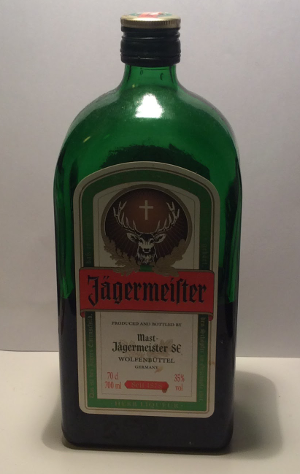
\includegraphics[width = 0.3\textwidth]{bottle.png}} &
\subfloat[Grayscale image]{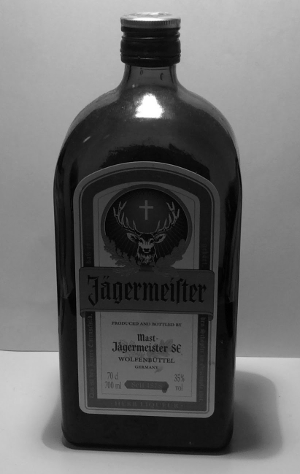
\includegraphics[width = 0.3\textwidth]{results/bottle-gray}} &
\subfloat[Gradient angles]{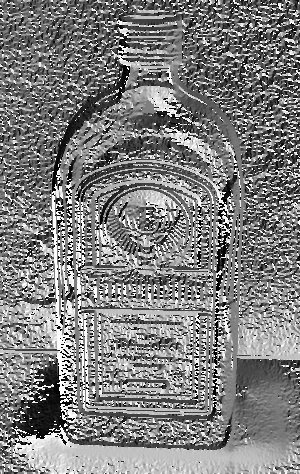
\includegraphics[width = 0.3\textwidth]{results/bottle-gradient-angles}} \\

\subfloat[Gradient magnitudes]{
\includegraphics[width = 0.3\textwidth]{results/bottle-gradient-magnitudes}} &
\subfloat[Non-maxima thinned edges]{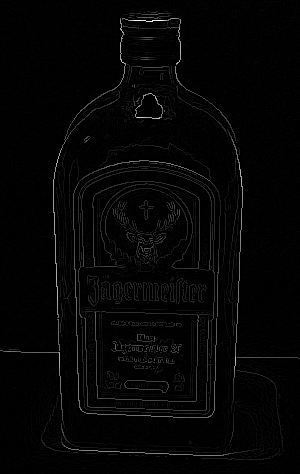
\includegraphics[width = 0.3\textwidth]{results/bottle-thinned}} &
\subfloat[Hysteresis chained edges]{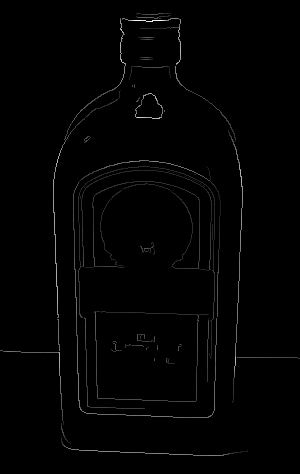
\includegraphics[width = 0.3\textwidth]{results/bottle-thinned_hyst}} \\

\end{tabular}
\caption{Results of the Canny edge detection phase}
\label{fig:attacks}
\end{figure}

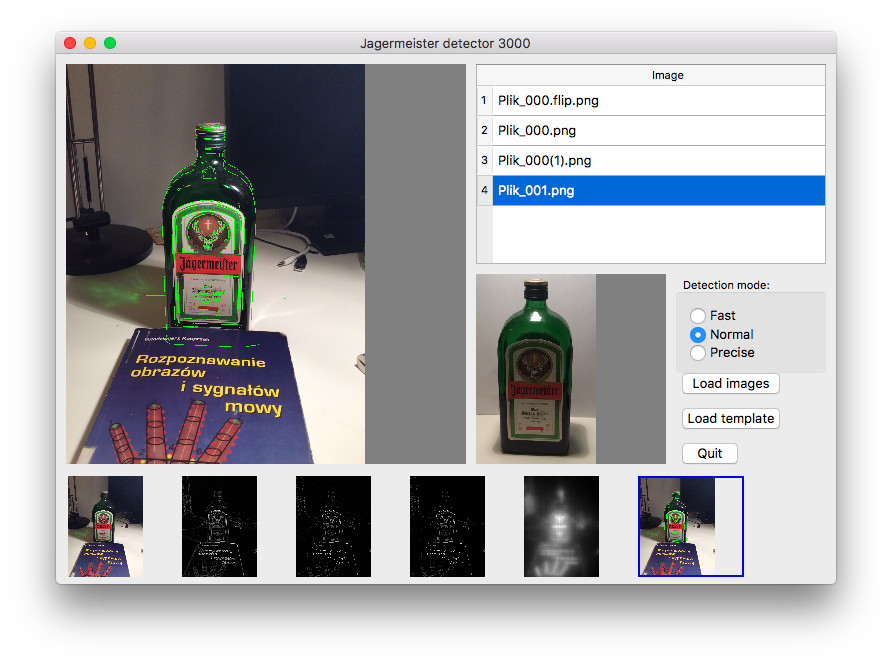
\includegraphics[width = 0.6\textwidth]{ui}

\section{Conclusions}

In our tests we succesfully craeted a model of a bottle shape based on a cropped image and detected
said bottle in several test images.

We found out that the number of possible discrete values of rotation and scaling greatly affects
the quality of results but also performance.  We had to tune the number of scalings to just 6 to
achieve acceptable runtime, which caused some instances to not be detected.


\end{document}
